\documentclass[a4paper]{article}
\frenchspacing

\def\tup#1{\langle#1\rangle}

%% Language and font encodings
\usepackage[english]{babel}
\usepackage[utf8]{inputenc}
\usepackage[T1]{fontenc}
\usepackage[autostyle]{csquotes}
\usepackage[ocgcolorlinks,pdfusetitle]{hyperref}
\usepackage{tikz}
\usetikzlibrary{graphs,graphs.standard}
\usetikzlibrary{positioning}
\tikzset{main node/.style={circle,fill=blue!20,draw,minimum size=1cm,inner sep=0pt},}
% for doi link
\usepackage{doi}

%% Sets page size and margins
\usepackage[a4paper,top=3cm,bottom=2cm,left=3cm,right=3cm,marginparwidth=1.75cm]{geometry}
% * <patric.fulop@gmail.com> 2016-11-23T00:32:01.744Z:
%
% ^.
%% Useful packages
\usepackage{amsmath,amssymb}
\usepackage{txfonts}
\usepackage{graphicx}

\usepackage[colorinlistoftodos]{todonotes}
%\usepackage{biblatex}
\usepackage{natbib}
\usepackage{authblk}
\usepackage{mathrsfs}
\usepackage{subcaption}
\usepackage{float}
\bibliographystyle{alpha}
\DeclareMathOperator{\E}{\mathbb{E}}
\DeclareMathOperator{\p}{\textbf{p}}
\DeclareMathOperator{\q}{\textbf{q}}
\DeclareMathOperator{\W}{\mathbb{W}}
\DeclareMathOperator{\boldH}{\textbf{H}}
\DeclareMathOperator{\boldV}{\textbf{V}}
\DeclareMathOperator{\boldX}{\textbf{X}}
\DeclareMathOperator{\boldY}{\textbf{Y}}
\DeclareMathOperator{\boldx}{\textbf{x}}
\DeclareMathOperator{\boldy}{\textbf{y}}
\DeclareMathOperator{\boldB}{\textbf{B}}
\DeclareMathOperator{\R}{\mathbb{R}}
\DeclareMathOperator{\boldh}{\textbf{h}}
\DeclareMathOperator{\boldv}{\textbf{v}}
\DeclareMathOperator{\arrow}{\rightsquigarrow}
\DeclareMathOperator{\daggerf}{f^{\dagger}}
\DeclareMathOperator{\daggerT}{T^{\dagger}}
\DeclareMathOperator{\bra}{\langle}
\DeclareMathOperator{\ket}{\rangle}
\DeclareMathOperator{\alphastar}{\alpha^*}
\DeclareMathOperator{\xprime}{x'}
\DeclareMathOperator{\wdata}{\W(\p_d,\p_\theta)}
\DeclareMathOperator{\wempirical}{\W_\gamma(\hat{\p},\p_\theta)}
\DeclareMathOperator{\klempirical}{KL({\hat{\p} || \p_\theta})}
\DeclareMathOperator{\kldata}{KL({\p_d || \p_\theta})}
\bibliographystyle{alpha}

\newtheorem{lemma}{Lemma}
\title{ICM Collaboration Notes}
\author{Patric Fulop \& Alex Agachi}
%{s1043702@sms.ed.ac.uk}
\affil{The University of Edinburgh}

\begin{document}
\maketitle


\section{Introduction}
Identify potential, explain problem, literature review, explain briefly what you're predicting in light of lit review. Then conclude by using different benchmarks. 
\section{Data statistics}
There are two main datasets, one with biological information and one with clinical data. 
We give a brief description of the merged dataset before preprocessing:
%
\begin{itemize}
\item \textbf{Key 1:} Patient ID - this is not unique across rows
\item \textbf{Key 2:} Surgery date and clinical surgery date. 
These are sometimes off by one day so we took only surgery dates as being relevant.
\end{itemize}
%
There are a total of \textbf{7825} entries and \textbf{6688} unique patients. Each patient has \textbf{30} relevant attributes. For convenience, the attribute names have been renamed more intuitively, and in English :). \\
\\
Some of the attributes have missing values.
\begin{enumerate}
\item Diagnostic dates are there only for one fifth of the patients,  \textbf{1162}.
\item Date of birth (DoB) is missing for \textbf{1002} patients.
\item Date of death is missing for \textbf{4908} entries, should we assume these are survivors? 
\item Gene data is very sparse, i.e. \textbf{Ch} markers.
\item Gender data has \textbf{332} entries missing.
\end{enumerate}

%\subitem IDHmut>IDHwt - 2 classes 
%\subitem Codel >IDHmut> IDHwt (3 classes)
%\subitem IDHmut-Tertmut>IDHmu-Tertwt>IDHwtTertwt>IDHwtTertmut (4 classes)

%MGMTm -binary
%P16 loss binary 
%EGFR amplitude - binary 
 %Loss Chr10 - binary 


\begin{table}[tb]
\vskip 3mm
\begin{center}
\begin{small}
\begin{sc}
\begin{tabular}{lcccr}
\hline
%\abovespace\belowspace
Attribute & Present & Missing & Encoding &Type \\
\hline
%\abovespace  \\
Age at surgery & to see & to see& Age & Numerical discrete  \\%Age at chemo
Gender  & 7493 & 332 & Gender & Binary\\
Histo Grade    & 7825& 0&  Tumor Grade & Categorical (4)      \\
Histo Type    & 7825& 0&  Tumor Type & Categorical   \\
KPS    & ?& ?&  ?  &?    \\
Outcome & 4766 & 3059 & Surgery Type & Categorical (3)\\
Radiotherapy    & 2722& 5103&  Rx Date  & Time $\to$ Ultimately Binary \\
Chemotherapy   & 2950& 4875&  Chemo Date  &Time $\to$ Ultimately Binary    \\
IDH Mutation 1   & 7327& 498&  Gene IDH1 & Categorical (3)   \\
IDH Mutation 2   &7078 & 747&  Gene IDH2   & Categorical (3) \\
Htert C228T & 4336 & 3489 & Gene C228T & Categorical (3)\\ 
Htert C250T & 4333 & 3492 & Gene C250T  & Categorical (3) \\ 
%\belowspace
\hline
\end{tabular}
\end{sc}
\end{small}
\caption{Present and missing variables and their encoding}
\label{tab:encoding}
\end{center}
\vskip -3mm
\end{table}

\section{Encoding clarifications and target variables}
As previously discussed, in the first phase we are interested in a smaller subset of attributes. Table \ref{tab:encoding} above indicates some of the variables of interest. Please let us know if we got the right ones and whether we should add more from the dataset. \\
For some of them, some things remain unclear. \\
\begin{enumerate}
\item We aim to add age at surgery as one variable, taking into account surgery date and date of birth. 
\item We do not have any attribute for KPS (performance status score) as far as we know. 
\item The outcome is encoded in the surgery type variable \ref{fig:sub1}. It is either a type of surgical removal or biopsy. For this variable, does missing data tell us that there was no surgery or that we do not know the outcome?
Does \textbf{aucune} mean that no surgical act whatsoever was undertaken?
\item For radiotherapy and chemotherapy, should we assume that if the patient does not have a date, he did not undergo that treatment, or is this data missing instead? 
\item For IDH mutations \ref{fig:sub2}, IDH1 and IDH2 seem to predominate there. Are these the two main ones we are interested in? You mentioned IDH wild type/mutated, so we concluded the \textbf{NORMAL} value of IDH1/IDH2 Gene stands for wild-type. Is this correct? In this context, what does the value \textbf{NC} stand for?
\item In terms of genetic tests, is there any equivalence between the following coding schemes for various genes, i.e. can we treat \textbf{NORMAL} or \textbf{ALTERE} as carrying the same meaning across these schemes/genes? i.e. \ref{fig:sub2}, \ref{fig:sub3} and \ref{fig:sub4}.
\end{enumerate}
%%% IMAGE 1  
\begin{figure}[H]
\centering
\begin{subfigure}{.2\textwidth}
  \centering
  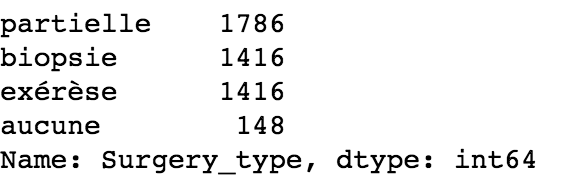
\includegraphics[width=1.0\linewidth]{images/Surgery_type.png}
  \caption{Surgery Type}
  \label{fig:sub1}
\end{subfigure}%
\begin{subfigure}{.2\textwidth}
  \centering
  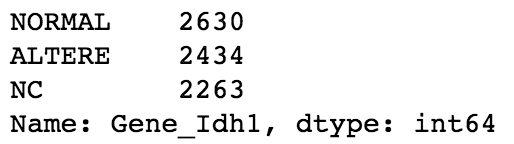
\includegraphics[width=1.0\linewidth]{images/Gene_Idh1.png}
  \caption{Gene Idh1}
  \label{fig:sub2}
\end{subfigure}%
\begin{subfigure}{.2\textwidth}
  \centering
  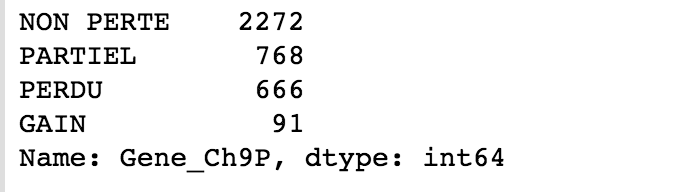
\includegraphics[width=1.0\linewidth]{images/Gene_Ch9P.png}
  \caption{Gene Ch9P}
  \label{fig:sub3}
\end{subfigure}
\begin{subfigure}{.2\textwidth}%
  \centering
  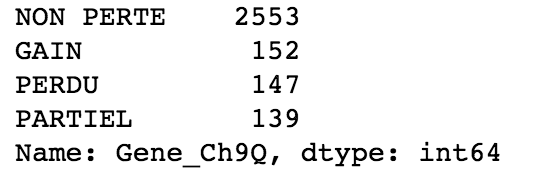
\includegraphics[width=1.0\linewidth]{images/Gene_Ch9Q.png}
  \caption{Gene Ch9Q}
  \label{fig:sub4}
\end{subfigure}
\caption{Outcome and Gene Mutations}
\label{fig:genes}
\end{figure}
%
\textbf{Multiple entries:} On average, patients have more than 1 entry (see fig. \ref{fig:m_entries}) according to how many surgeries they went through. Is that correct and do you have any pointers as to how to treat patients with multiple surgeries? Should we aggregate them or treat them independently? Or perhaps find some other clever way of dealing with that. 
\begin{figure}[H]
\centering
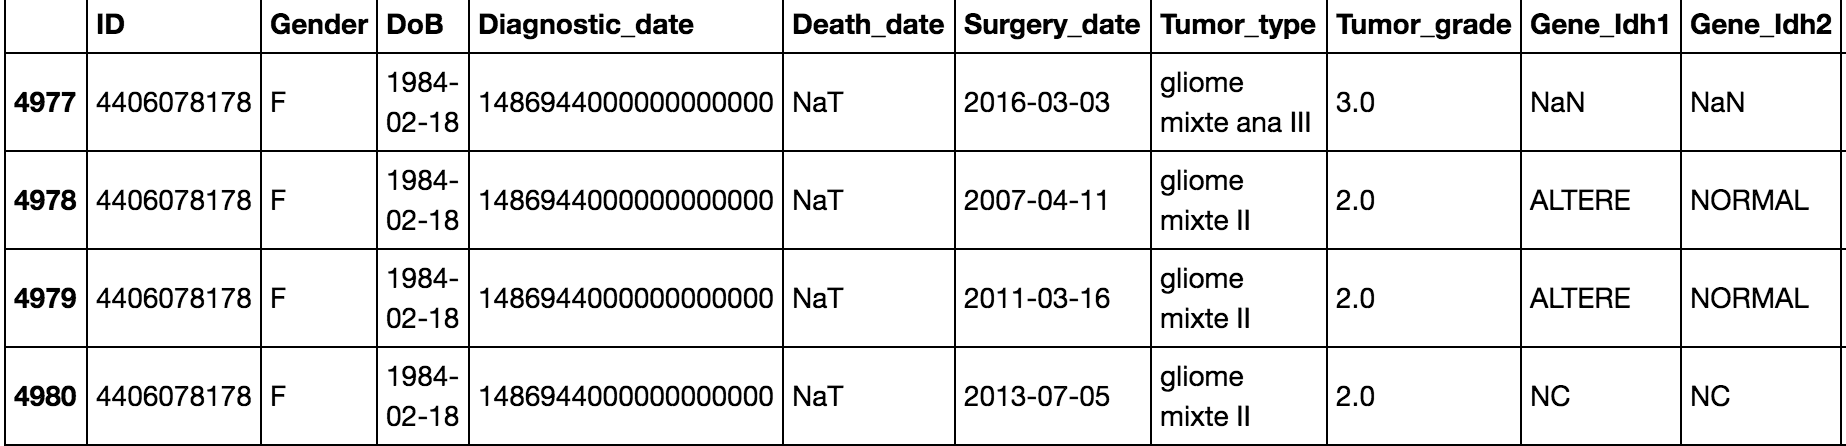
\includegraphics[width=1.0\linewidth]{images/multiple_entries.png}
\caption{Entries for patient 4406078178}
\label{fig:m_entries}
\end{figure}
% 
\textbf{Target Variable:}
We want to confirm our idea of selecting the target variable for our models. 
First of all, can we assume that all patients where there is no death date specified, are still alive? (as opposed to them not being alive anymore, but this record missing)
Qualitatively we thought of incorporating the surgery date, cancer detection date and death date, but we would much prefer if you would confirm. 
\begin{itemize}
\item The easiest target to model is a binary variable representing alive/dead.
\item The time between diagnostic date and death date. We would scale this variable accordingly to account for no death. 
\item The time between the first/last surgery and death time. We could incorporate in this the number of surgeries a person had. 
\end{itemize}
% \textbf{Feature standardization and class imbalances}
%
%Normal, Amplified
%Normal, increased, decreased, partial, 
%

\section{Literature Review}
We conducted a more focused meta study in the past, of studies tailored to datasets and target variables such as ours. We broke down the study among the important features: datasets used, machine learning models used, validation mechanisms and  feature engineering. 
Following this review, a possible first study on our dataset would include refining the following models:
\begin{itemize}
\item Clustering classifiers such as Gaussian Mixture models (GMM) 
\item Support Vector Machines (SVM)
\item Decision Trees 
\item Neural Networks
\end{itemize}
We would then compare the results across all four criteria commonly used: accuracy, sensitivity, specificity, ROC curve and area under the curve (AUC). A similar development was tackled by Garcia-Laencina et. al. (2015) \cite{Garcia-Laencina2015}, in which they focused on breast cancer. 
%%%% Missing data
\subsection{Dealing with Missing data}
Traditional techniques of dealing with missing data in medical studies, available case analysis, pairwise deletion, and single imputation are suboptimal and lead to either/both of loss of statistical power and increased bias in the results \cite{Bell2014}, \cite{Little2012}. As such, dealing with missing data in our study in a statistically robust manner has been a key area of focus in our data preparation to date.\\
\\
Clearly some patients in this dataset underwent some tests, while others did not. This is a problem we can deal with in a very robust manner as long as we can assume that the data is missing at random. The missing data mechanism relates to why values are missing and the connection of those reasons with treatment outcomes \cite{Garcia-Laencina2015}. Can we assume that these are random in our study? \\
\\
More concretely, for \textbf{C228T} we have \textbf{3489} missing observations in our dataset. Can we assume that these observations are missing in a way that is not reflective of the patients condition and outcome i.e. doctors simply did not order this test, or this test was not available at a specific time, all independent of the patient?s condition. Or if the data is not missing at random - for example the patients for whom we do not have the results to this test were significantly more ill-suffering from a more aggressive form of cancer than the ones for whom we do have the results? It would help to understand the mechanisms better, to make sure our methods are sound. We narrowed down here on a technique called multiple imputation (MI) by chained equations \cite{Graham2007}, \cite{Graham2009}. This type of imputation method involves replacing missing values by suitable estimates and then applying standard complete-data methods to the filled-in data. The basics ideas of MI as proposed by Rubin \cite{Rubin1996} involves the following three steps: 
\begin{enumerate}
\item Imputation: Impute missing values using an appropriate model that incorporates appropriate random variation. During this first step, sets of plausible values for missing observations are created that reflect uncertainty about the non-response model. These sets of plausible values can then be used M times to ?complete? the missing values and create M ?completed? data sets. 
\item Analysis: Perform the desired analysis on each of these M data sets using standard complete-data methods. 
\item Combination: During this final step, the results are combined, which allows the uncertainty regarding the imputation to be taken into account.
\end{enumerate}
%%%% 
%%% Feature Engineering
\subsection{Feature engineering}
Feature engineering (changing variables for example in terms of scale, or creating interaction variables?) is a very large part of building more accurate models. We already thought of adding extra variables based on the current ones, i.e. the time from diagnostic date to surgery (to check the effects of patients delaying significantly recommended surgeries) and the age at diagnostic. Are there other obvious ones you suspect? 


\bibliography{ICM}
\end{document}